\documentclass[12pt]{article}
\usepackage[letterpaper,total={7in,10in}]{geometry}
\usepackage{tikz}
\usepackage{ragged2e}
\usepackage{listings}
\usepackage{color}
\usepackage{multicol}
\renewcommand{\ttdefault}{txtt}
\renewcommand{\familydefault}{\ttdefault}
\begin{document}
	\Centering \huge \textbf{\underline{Programming Dictionary}}

	\Large By Charles Cook

	\large Begun on Dec. 6th, 2018

	\FlushLeft \large \section{Compiler Theoretical Foundations}

	\Centering 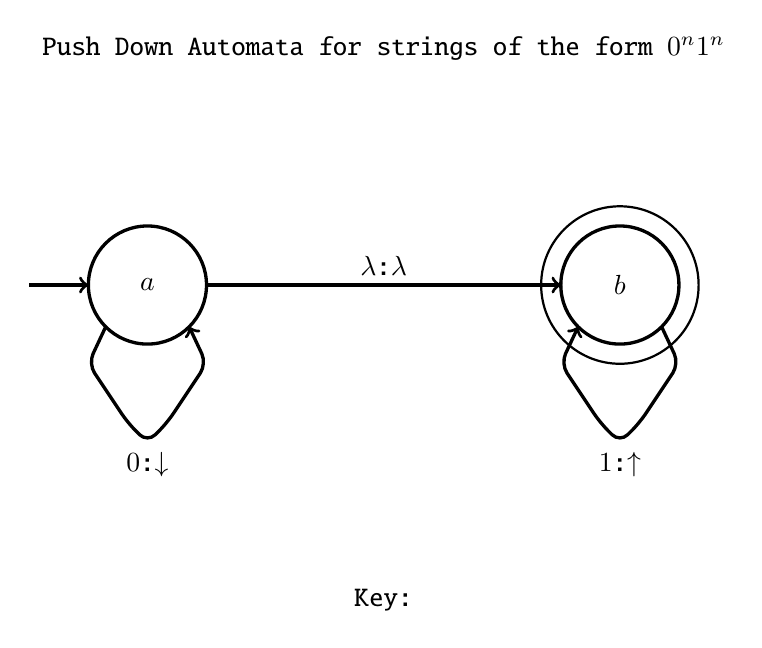
\begin{tikzpicture}
		\node at (0, 3) {Push Down Automata for strings of the form $0^n1^n$};
		\draw [very thick, ->] (-4.5, 0) -- (-3.75, 0);
		\draw [very thick] (-3, 0) circle (0.75);
		\node at (-3, 0) {$a$};
		\draw [very thick, rounded corners, ->] (-3.53, -0.53) -- (-3.75, -1) -- (-3.25, -1.75) -- (-3, -2) -- (-2.75, -1.75) -- (-2.25, -1) -- (-2.47, -0.53);
		\node [below] at (-3, -2) {$0$:$\downarrow$};
		\draw [very thick, ->] (-2.25, 0) -- (2.25, 0);
		\node [above] at (0, 0) {$\lambda$:$\lambda$};
		\draw [very thick] (3, 0) circle (0.75);
		\draw [thick] (3, 0) circle (1);
		\node at (3, 0) {$b$};\draw [very thick, rounded corners, ->] (3.53, -0.53) -- (3.75, -1) -- (3.25, -1.75) -- (3, -2) -- (2.75, -1.75) -- (2.25, -1) -- (2.47, -0.53);
		\node [below] at (3, -2) {$1$:$\uparrow$};
		\node at (0, -4) {Key:};
	\end{tikzpicture}

	\begin{tabular}{|l||r|}
		\hline Symbol & Meaning \\ \hline
		$a$, $b$ & State Node \\ \hline
		$0$, $1$ & Symbol to Print \\ \hline
		$\downarrow$ & Push (onto the stack) \\ \hline
		$\uparrow$ & Pull (off of the stack) \\ \hline
		$\lambda$ & Null operation \\ & (no print, push, or pull) \\ \hline
	\end{tabular}
	\pagebreak

	\FlushLeft \normalsize
	\section{Programming Tools \& Languages: First Ten Questions}
	\subsection{Swap Function}
	\subsubsection{Pseudocode for \textit{swap}}
	\begin{lstlisting}[language = C, tabsize = 8]
void swap(a, b) {
	temp = a;
	a = b;
	b = temp;
}

void swapNoTemp(a, b) {
	a += b; // a = a + b
	b -= a; // b = b - (a + b) = -a
	b *= -1; // b = a
	a -= b; // a = a + b - a = b
}
	\end{lstlisting}

	\subsubsection{\textit{swaptest.c}}
	\begin{lstlisting}[language = C, showstringspaces = false, tabsize = 8]
#include <stdio.h>
void swap(int *a, int *b) {
	*a += *b;
	*b -= *a;
	*b *= -1;
	*a -= *b;
}

int main() {
	int x, y, z;
	x = 10;
	y = 13;
	z = 2;

	swap(&x, &y);
	swap(&x, &z);
	swap(&y, &z);
	printf("x: &d\ny: &d\nz: &d\n", x, y, z);

	return 0;
}
	\end{lstlisting}
	\pagebreak
	\subsubsection{\textit{swaptest.cpp}}
	\begin{lstlisting}[language = C++, showstringspaces = false, tabsize = 8]
#include <iostream>
using namespace std;

void swap(int *a, int *b) {
	*a += *b;
	*b -= *a;
	*b *= -1;
	*a -= *b;
}

int main() {
	int x, y;
	x = 13;
	y = 29;

	cout << x << ", " << y << "\n";
	swap(x, y);
	cout << x << ", " << y << "\n";

	return 0;
}
	\end{lstlisting}

	\subsection{Reverse an array with no extra space (pseudocode)}
	\begin{lstlisting}[language = C, showstringspaces = false, tabsize = 8]
void reverseArray(array, int length) {
	for (int i = 0; i < length / 2; i++) {
		swap(array[i], array[length - i - 1]);
	}
}
	\end{lstlisting}

	\subsection{Reverse a doubly linked list (pseudocode)}
	\begin{lstlisting}[language = C, showstringspaces = false, tabsize = 8]
struct Node {
	int data;
	struct Node *next;
	struct Node *prev;
};

void reverseDLL(head, tail) {
	struct Node tempH = head;
	struct Node tempT = tail;

	while (tempH -> next != tempT -> prev && tempH != tempT) {
		swap(tempH -> data, tempT -> data);
	}
}
	\end{lstlisting}
	\subsection{Reverse a doubly linked list recursively (pseudocode)}
	\begin{lstlisting}[language = C, showstringspaces = false, tabsize = 8]
void reverseDLL_Recursive(head, tail) {
	if (head -> next != tail -> prev && head != tail) {
		swap(head -> data, tail -> data);
		reverseDLL_Recursive(head -> next, tail -> prev);
	}
}
	\end{lstlisting}
\end{document}
